\Chapter{Tervezés}

Mielőtt eljutunk egy kész modellig rengeteg minden történik. Először is ezeket a lépéseket szeretném ismertetni ebben a fejezetben. Utána bemutatnám az adathalmazt amivel dolgoztam. Végül pedig a különféle gépi tanulói algoritmusokat amiket használtam dolgozatom során.

\Section{Folyamat ismertetése}
\begin{enumerate}
    \item Adatok összegyűjtése: Ahhoz, hogy el tudjuk kezdeni a munkát valahonnan adatokat kell szerezni. Ezt megtehetjük magunk is online oldalak után kutatva, aminek a tartalmát web scraping segítségével egy számunkra kedvező adattípusú fájlba le lehet menteni, mint pélául JSON, CSV.
    \item Adatok előkészítése: Miután megvan az adathalmazom meg kell vizsgálni, hogy nincs-e benne olyan adatrész, ami később negatívan befolyásolhatja a modellem pontosságát. Ilyenek lehetnek az üres sorok, szám helyett szöveg van beírva, esetleg teljesen értelmetlen dolog került az adatok közé. Ezeket természetesen valamilyen módon orvosolni kell. Arról, hogy ezeket a hibákat hogyan lehet kijavítani egy későbbi fejezetben fogok írni.
    \item Adatelemzés: Ez a lépés azért szükséges, hogy közelebb kerüljek az adathalmaz megértéséhez, mintákat fedezzek fel benne, esetleg olyan anomáliákat, amik eddig nem tűntek fel. Változók között összefüggéseket lehet találni. Valamint megállapítani azokat a változókat, amik leginkább befolyásolni fogják a modellem pontosságát.
    \item Modell tanítása és elemzése: Mivel többféle algoritmus is létezik először ezeket mind be kell tanítani, hogy az adott feladatot el tudják végezni. Ezt követően meg kell nézni egy tesztelés céljára létrehozott adathalmazzal, hogy melyik milyen eredményeket ér el, és ez alapján dönteni, hogy végső soron melyik tudja legjobban ellátni a rábízott feladatot \cite{machinelearningbasics}. 
\end{enumerate}

\Section{Adathalmaz bemutatása}
Mivel adathalmaz egy online kutatásból elérhető amit Nuno Antonio, Ana Almeida és Luis Nunes csinált 2019 februárjában, ezért a folyamat első lépésén túl is vagyunk. Az adathalmazt kaggle.com-ról töltöttem le. Szállodafoglalási adatokat tartalmaz, egy városi szállodáról és egy üdülőszállóról. Mindkét szálloda esetében 32 különböző változó található, amiből 31 jelleg változó, 1 pedig a kimeneti változó, összesen közel 120.000 mintával.\cite{adathalmaz}

A változók a következőek:
\begin{itemize}
    \item \textbf{hotel:} A hotel típusát adja meg, azaz városi szálloda vagy üdülőszálló. 
    
    Adattípus: kategorikus adat
    \item \textbf{lead\_time:} Hány nappal hamarabb foglalták le a szállást mint ahogy érkeznek. 
    
    Adattípus: egész szám
    \item \textbf{arrival\_date\_year:} Melyik évben érkezik a vendég a szállásra. 
    
    Adattípus: egész szám
    \item \textbf{arrival\_date\_month:} Melyik hónapban érkezik a vendég a szállásra. 
    
    Adattípus: egész szám
    \item \textbf{arrival\_date\_week\_number:} Hanyadik héten érkezik a vendég a szállásra. 
    
    Adattípus: egész szám
    \item \textbf{arrival\_date\_day\_month:} Hanyadik napon érkezik az adott hónapban a vendég a szállásra. 
    
    Adattípus: egész szám
    \item \textbf{stays\_in\_weekend\_nights:} Hány hétvégi éjszakát (szombat, vasárnap) marad/foglalt a vendég. 
    
    Adattípus: egész szám
    \item \textbf{stays\_in\_week\_nights:} Hány hétköznapi éjszakát (hétfőtől, péntekig) marad/foglalt a vendég. 
    
    Adattípus: egész szám
    \item \textbf{adults:} Felnőttek száma. 
    
    Adattípus: egész szám
    \item \textbf{children:} Gyerekek száma. 
    
    Adattípus: egész szám
    \item \textbf{babies:} Babák száma. 
    
    Adattípus: egész szám
    \item \textbf{meal:} Milyen étkezést foglalt a vendég (reggeli, félpanzió, teljes ellátás). 
    
    Adattípus: kategorikus adat
    \item \textbf{country:} Milyen országból származik a vendég. 
    
    Adattípus: szöveg
    \item \textbf{market\_segment:} Milyen piaci szegmensből érkezett a foglalás (online/offline utazási irodán keresztül, direkt szállódával stb.). 
    
    Adattípus: szöveg
    \item \textbf{distribution\_channel:} Milyen csatornán keresztül foglaltak (utazási iroda, direkt szállódával stb). 
    
    Adattípus: szöveg
    \item \textbf{is\_repeated\_guest:} Visszajáró vendég-e. 
    
    Adattípus: logikai érték
    \item \textbf{previous\_cancellations:} Hány foglalást mondott le előzőleg az adott szállodánál a vendég. 
    
    Adattípus: egész szám
    \item \textbf{previous\_bookings\_not\_canceled:} Hány foglast nem mondott le a vendég az adott szállodánál. 
    
    Adattípus: egész szám
    \item \textbf{reserved\_room\_type:} A foglalt szoba típusa. 
    
    Adattípus: szöveg
    \item \textbf{assigned\_room\_type:} A kapott szoba típusa. 
    
    Adattípus: szöveg
    \item \textbf{booking\_changes:} Hányszor módosították a foglalást a megérkezésig. 
    
    Adattípus: egész szám
    \item \textbf{deposit\_type:} Fizetett-e előleget a vendég. 3 lehetőség van, nem fizetett, fizetett de visszakaphatja, fizetett és nem kaphatja vissza. 
    
    Adattípus: kategorikus adat
    \item \textbf{agent:} Az utazási iroda ID-ja amin keresztül a foglalt a vendég. 
    
    Adattípus: szöveg
    \item \textbf{company:} A cég ID-je amin keresztül foglaltak és aki felelős azért, hogy ki legyen fizetve a szállás. 
    
    Adattípus: szöveg
    \item \textbf{days\_in\_waiting\_list:} A napok száma mielőtt visszaigazoltak egy foglalást.
    
    Adattípus: egész szám
    \item \textbf{customer\_type:} Milyen típusú a foglalás. 
    
    Adattípus: szöveg
    \item \textbf{adr:} Napi átlagár. 
    
    Adattípus: lebegőpontos érték
    \item \textbf{required\_car\_parking\_spaces:} Hány parkolóhelyet kért a vendég. 
    
    Adattípus: egész szám
    \item \textbf{total\_of\_special\_requests:} Hány különleges kérése volt a vendégnek. 
    
    Adattípus: egész szám
\end{itemize}
Ez volt idáig a 31 jelleg változó, amiből a modellnek meg kell majd tudnia állapítani a kimenetet, ami 0 nem lemondott foglalás eseten, 1 pedig lemondott foglalás esetén.

Az egy kimeneti változó pedig:
\begin{itemize}
    \item \textbf{is\_canceled:} Le lett-e mondva a foglalás. 
    
    Adattípus: logikai érték
\end{itemize}

\Section{Gépi tanulási algoritmusok ismertetése}
Az adatok amin dolgozni fogunk címkézve vannak, amik a bemeneteket két lehetséges kimenetre választja szét, ami ugye a nem lemondott foglalás (0) és a lemondott foglalás (1).

Így a 3 fő technika közül a felügyelt tanulással foglalkozó algoritmusokra esett a választásom. Azonban ezen belül is kétfajta felügyelt tanulási módszer létezik az osztályozás és a regreszió. Az osztályozásban előre meghatázott osztályokba kell behelyezni a kimenetet, a regressziónál azonban egy folytonos értéktartományba kell behelyezni. A problémámban, mivel csak kétféle osztály van az osztályozási algoritmusok közül kell választani.

Ebből is rengeteg féle és fajta van. Szakdolgozatomban a következő öttel foglalkoztam a Scikit-learn könyvtárból.

\begin{itemize}
    \item Decision Tree Classifier (Döntési fa),
    \item Random Forest Classifier (Véletlen erdő),
    \item Logistic Regression (Logisztikus regresszió),
    \item K-nearest Neighbour Classifier (K-legközelebbi szomszédon alapuló osztályozás),
    \item Gradient Boosting Classifier.
\end{itemize}

\subsection{Decision Tree Classifier (Döntési fa)}
A döntési fa a különböző döntési lehetőségeket ábrázolja, az esetleges következményeket, esélyeket, hasznosságot és erőforrásokat figyelembe véve, attól függően, hogy mire használják. A döntési fa egy olyan faszerkezet, amelyben minden belső csúcs egy értékre vonatkozó ellenőrzést jelöl, a csúcsból kivezető minden él pedig az ellenőrzés egy-egy kimenetének feleltethető meg, így lehetővé téve, hogy fa formában ábrázoljunk függvényeket. Könnyen érthető, magyarázható; inkább értékek, mint függvények szerepelnek benne. Az induktív tanulási módszerek közé tartozik, és mindig csak egy eredményt ad magyarázattal, akkor is, ha több legjobb megoldás lenne. Érzékeny a tanulóhalmaz hibáira, és a további tanuláshoz újabb döntési fát kell generálni. Kombinálható más módszerekkel, így javítani lehet a hibáin. Egy lehetséges döntési fa látható a \ref{fig:dontesifa} ábrán.

A döntési fa előállítására több eljárást is kidolgoztak. Ezek mind rekurzív algoritmusok, amik egy kérdésre adott válasz szerint szétbontják a tanulóhalmazt. A kérdéseket úgy teszik fel, hogy a kisebb részek homogénebbek legyenek a magyarázandó változó szempontjából, mint az egész \cite{dontesi_fa_1}.

Több kritériumot is megadnak a rekurzió leállítására az egyes ágakon:
\begin{itemize}
    \item Nincs értelme tovább osztani a csomópont elemeit:
    \begin{itemize}
        \item A csomóponthoz tartozó elemek homogének a vizsgált tulajdonságokra.
        \item Elfogytak a csomóponthoz tartozó elemek.
        \item Elfogytak az osztályozó attribútumok.
    \end{itemize}
    \item Az adott ág elért egy bizonyos mélységet.
\end{itemize}

\subsubsection{A döntési fa előnyei:}
\begin{itemize}
    \item Egyszerű megérteni. A fákat vizualizálni is lehet.
    \item Nem igényli az adatok nagyszíntű előkészítését, azonban hiányzó adatokkal nem tud mit kezdeni.
    \item Az algoritmus számítási ideje logaritmikusan nő attól függően, hogy hány adat ponttal tanítottuk a modellt. Egy viszonlyag kis számítási idejű algoritmusról beszélünk.
    \item Képes kezelni mind a numerikus és mind a kategorikus adatokat, azonban a scikit-learn implementációja az algoritmusnak még nem támogatja a kategorikus változókat.
    \item Képes megoldani több kimenetű problémákat.
    \item White box modellt használ. Ami azt jelenti, hogy könnyen megérthető miért hozott egy adott döntést az algoritmus.
    \item Lehetséges igazolni a modellt statisztikai tesztekkel. Ezzel lehetővé téve, hogy megtudjuk mondani mennyire megbízható az adott modell.
\end{itemize}
\subsubsection{A döntési fa hátrányai:}
\begin{itemize}
    \item Az ilyen tanulási algoritmusok néha túl komplex fákat tudnak létrehozni amik nem általánosítják jól a rendelkezésre álló adatokat.
    \item A döntési fák bizonytalanok lehetnek, mert egy kis variáció is az adatban teljesen más fákat generálhat. Ezt úgy lehet csillapítani, hogyha több döntési fát egy csoportban használunk, és az egész csoportnak megnézni mi lesz a kimenete.
    \item Néhány dolgot, mint például a paritás vagy az XOR művelet nehéz megtanulnia, mivel ezeket a műveleteket a döntési fa nem egyszerű módon fejezi ki.
    \item Ha egy bizonyos kimeneti osztály dominál egy adathalmazon belül, akkor könnyen szubjektív lehet az algoritmus a domináns kimeneti osztály irányába. Ezért célszerű egyenlően megosztani kimeneti osztályok arányát a tanításra használt adathalmazon belül \cite{dontesi_fa_2}. 
\end{itemize}
\begin{figure}[h]
    \centering
    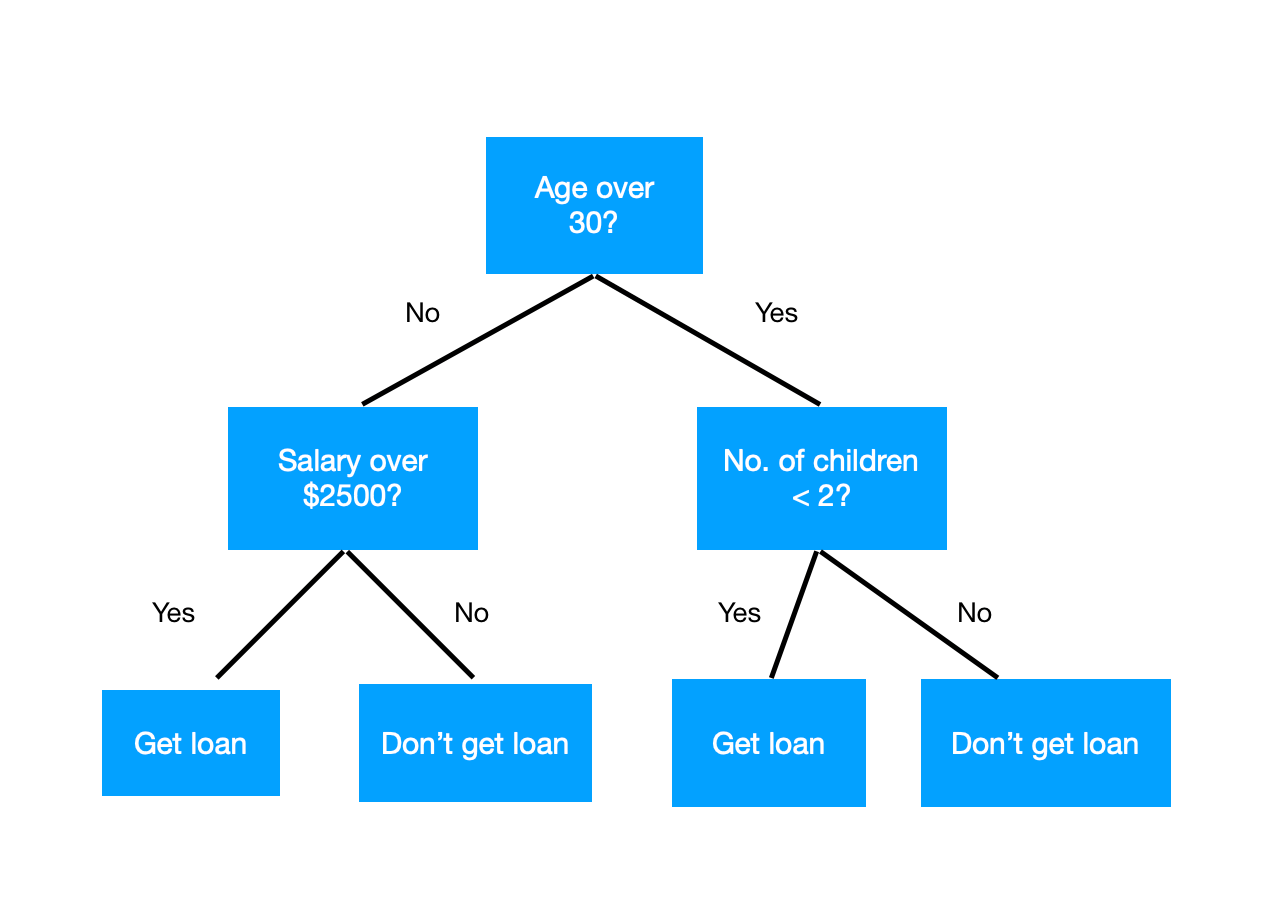
\includegraphics[width=\linewidth]{images/3.fejezet/DecisionTree.png}
    \caption{Döntési fa egy egyszerű példával szemléltetve \cite{dontesifa_abra}}
    \label{fig:dontesifa}
\end{figure}


\subsection{Random Forest Classifier (Véletlen erdő)}
A Random Forest vagy magyarul véletlen erdő egy gépi tanulásban használt klasszifikációs és regressziós módszer, aminek a lényege, hogy több különböző döntési fát hoz létre, és ezek eredményeinek átlagolásával vagy klasszifikáció esetén a legtöbb szavazatot kapott eredmény kiválasztásával adja meg a végeredményt. Egy lehetséges véletlen erdő látható a \ref{fig:veletlenerdo} ábrán.

Ahhoz, hogy a módszer jól működjön, az szükséges, hogy az egyes döntési fák a véletlennél jobban teljesítsenek, illetve hogy az előrejelzéseik, és így a hibáik egymástól viszonylag függetlenek legyenek, azaz kicsi legyen köztük a korreláció. A több döntési fa együttes alkalmazása így ki tudja szűrni az egyes döntési fák által vétett hibákat \cite{veletlen_erdo_1}.

\subsubsection{A véletlen erdő előnyei:}
\begin{itemize}
    \item Pontos becsléseket adó gépi tanulási algoritmus.
    \item Nagy adathalmazokra is használható gyors futása miatt.
    \item Sok dimenziójú bemenetet is képes kezelni.
    \item Megbecsülik melyik változók fontosak a modell szempontjából.
    \item A hiányzó adatok megbecsülésére is képes.
\end{itemize}

\subsubsection{A véletlen erdő hátrányai:}
\begin{itemize}
    \item A döntési fákkal ellentétben a véletlen erdőknél nehéz megmondani, hogy mi alapján hozta a döntését. Úgymond black box modellt használ.
    \item Túltanulásra hajlamos az algoritmus, ha nem teljesen egyértelmű az osztályozandó feladat. A túltanulás azt jelenti, hogy nem csak az általános információkat tanulja meg, hanem az adott adathalmaz sajátósságait is \cite{veletlen_erdo_3}.
\end{itemize}

\begin{figure}[h]
    \centering
    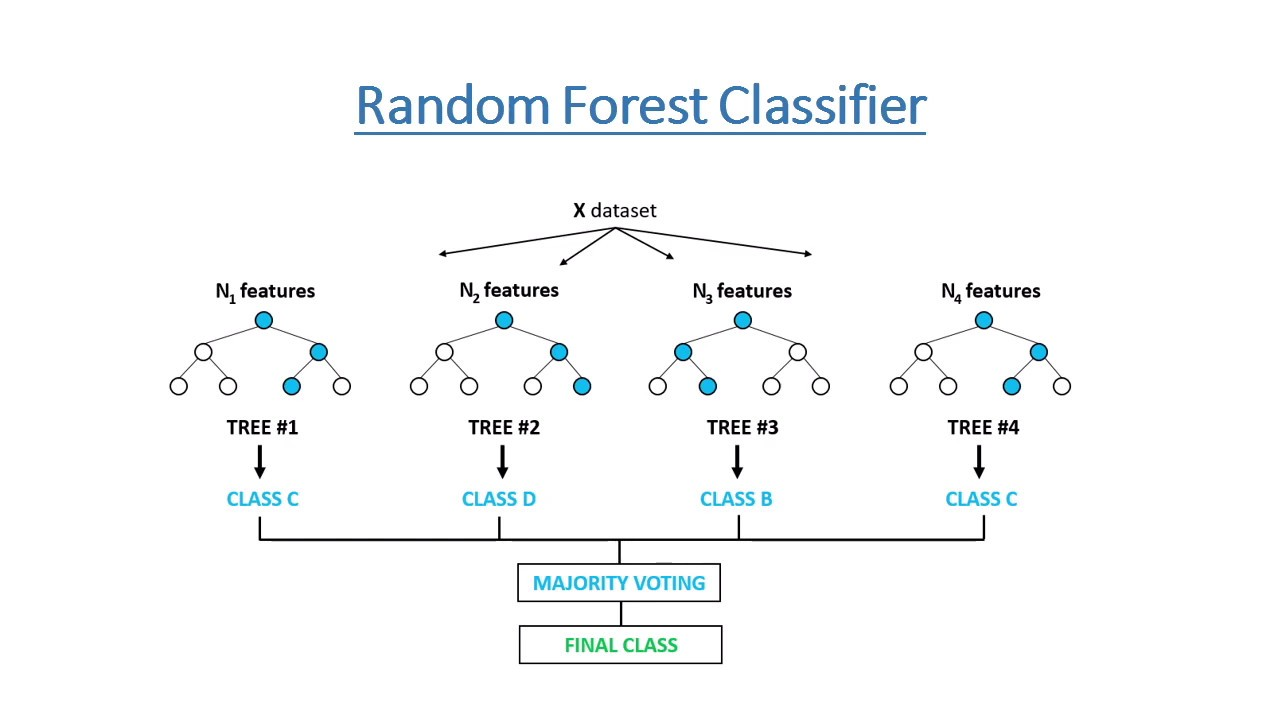
\includegraphics[width=\linewidth]{images/3.fejezet/RandomForest.jpg}
    \caption{Véletlen erdő egy egyszerű példával szemléltetve \cite{veletlenerdo_abra}}
    \label{fig:veletlenerdo}
\end{figure}



\subsection{Logistic Regression (Logisztikus regresszió)}
Egy algoritmus ami a lineáris regressziónak egy kiterjesztett változata osztályozásra. A lineáris regresszió által kapott értékeket átadja egy szigmoid függvénynek, ezáltal a kimeneti értékek 0 és 1 között lesznek.   Arra használják, hogy megadják egy esemény bekövetkezésének valószínűségét (Esetemben ez az esemény a szoba foglalás lemondása). Akkor célszerű használni ezt a módszert, amikor a kimenő adat kétértékű (pl.: 0/1, Igaz/Hamis, Igen/Nem) \cite{logisztikus_regresszio_2}. A \ref{fig:logisztikusregresszio} ábrán egy lehetséges logisztikus regresszió ábrázolása látható.

\subsubsection{Logisztikus regresszió előnyei:}
\begin{itemize}
    \item Egyszerű implementálni és megérteni.
    \item Nem számít, hogyha dominál egy kimeneti osztály. Így nem egyensúlyba lévő osztályokkal rendelkező adathalmazon is lehet tanítani.
    \item Jó pontossággal dolgozik egyszerű adatok esetén, különösen akkor ha az adathalmaz lineárisan elválasztható.
\end{itemize}

\subsubsection{Logisztikus regresszió hátrányai:}
\begin{itemize}
    \item Lineáris határokat állít az osztályok közé.
    \item Csak diszkrét kimenetek meghatározására használható.
    \item A nemlineáris feladatokat nem célszerű megoldani vele mivel a lineáris regressziónak köszönhetően csupán lineáris döntési felülete van.
    \item Nehéz olyan modellt építeni ezen algoritmus segítségével ami összetett problémák felett tudna dönteni \cite{logisztikus_regresszio_2}.
\end{itemize}

\begin{figure}[h]
    \centering
    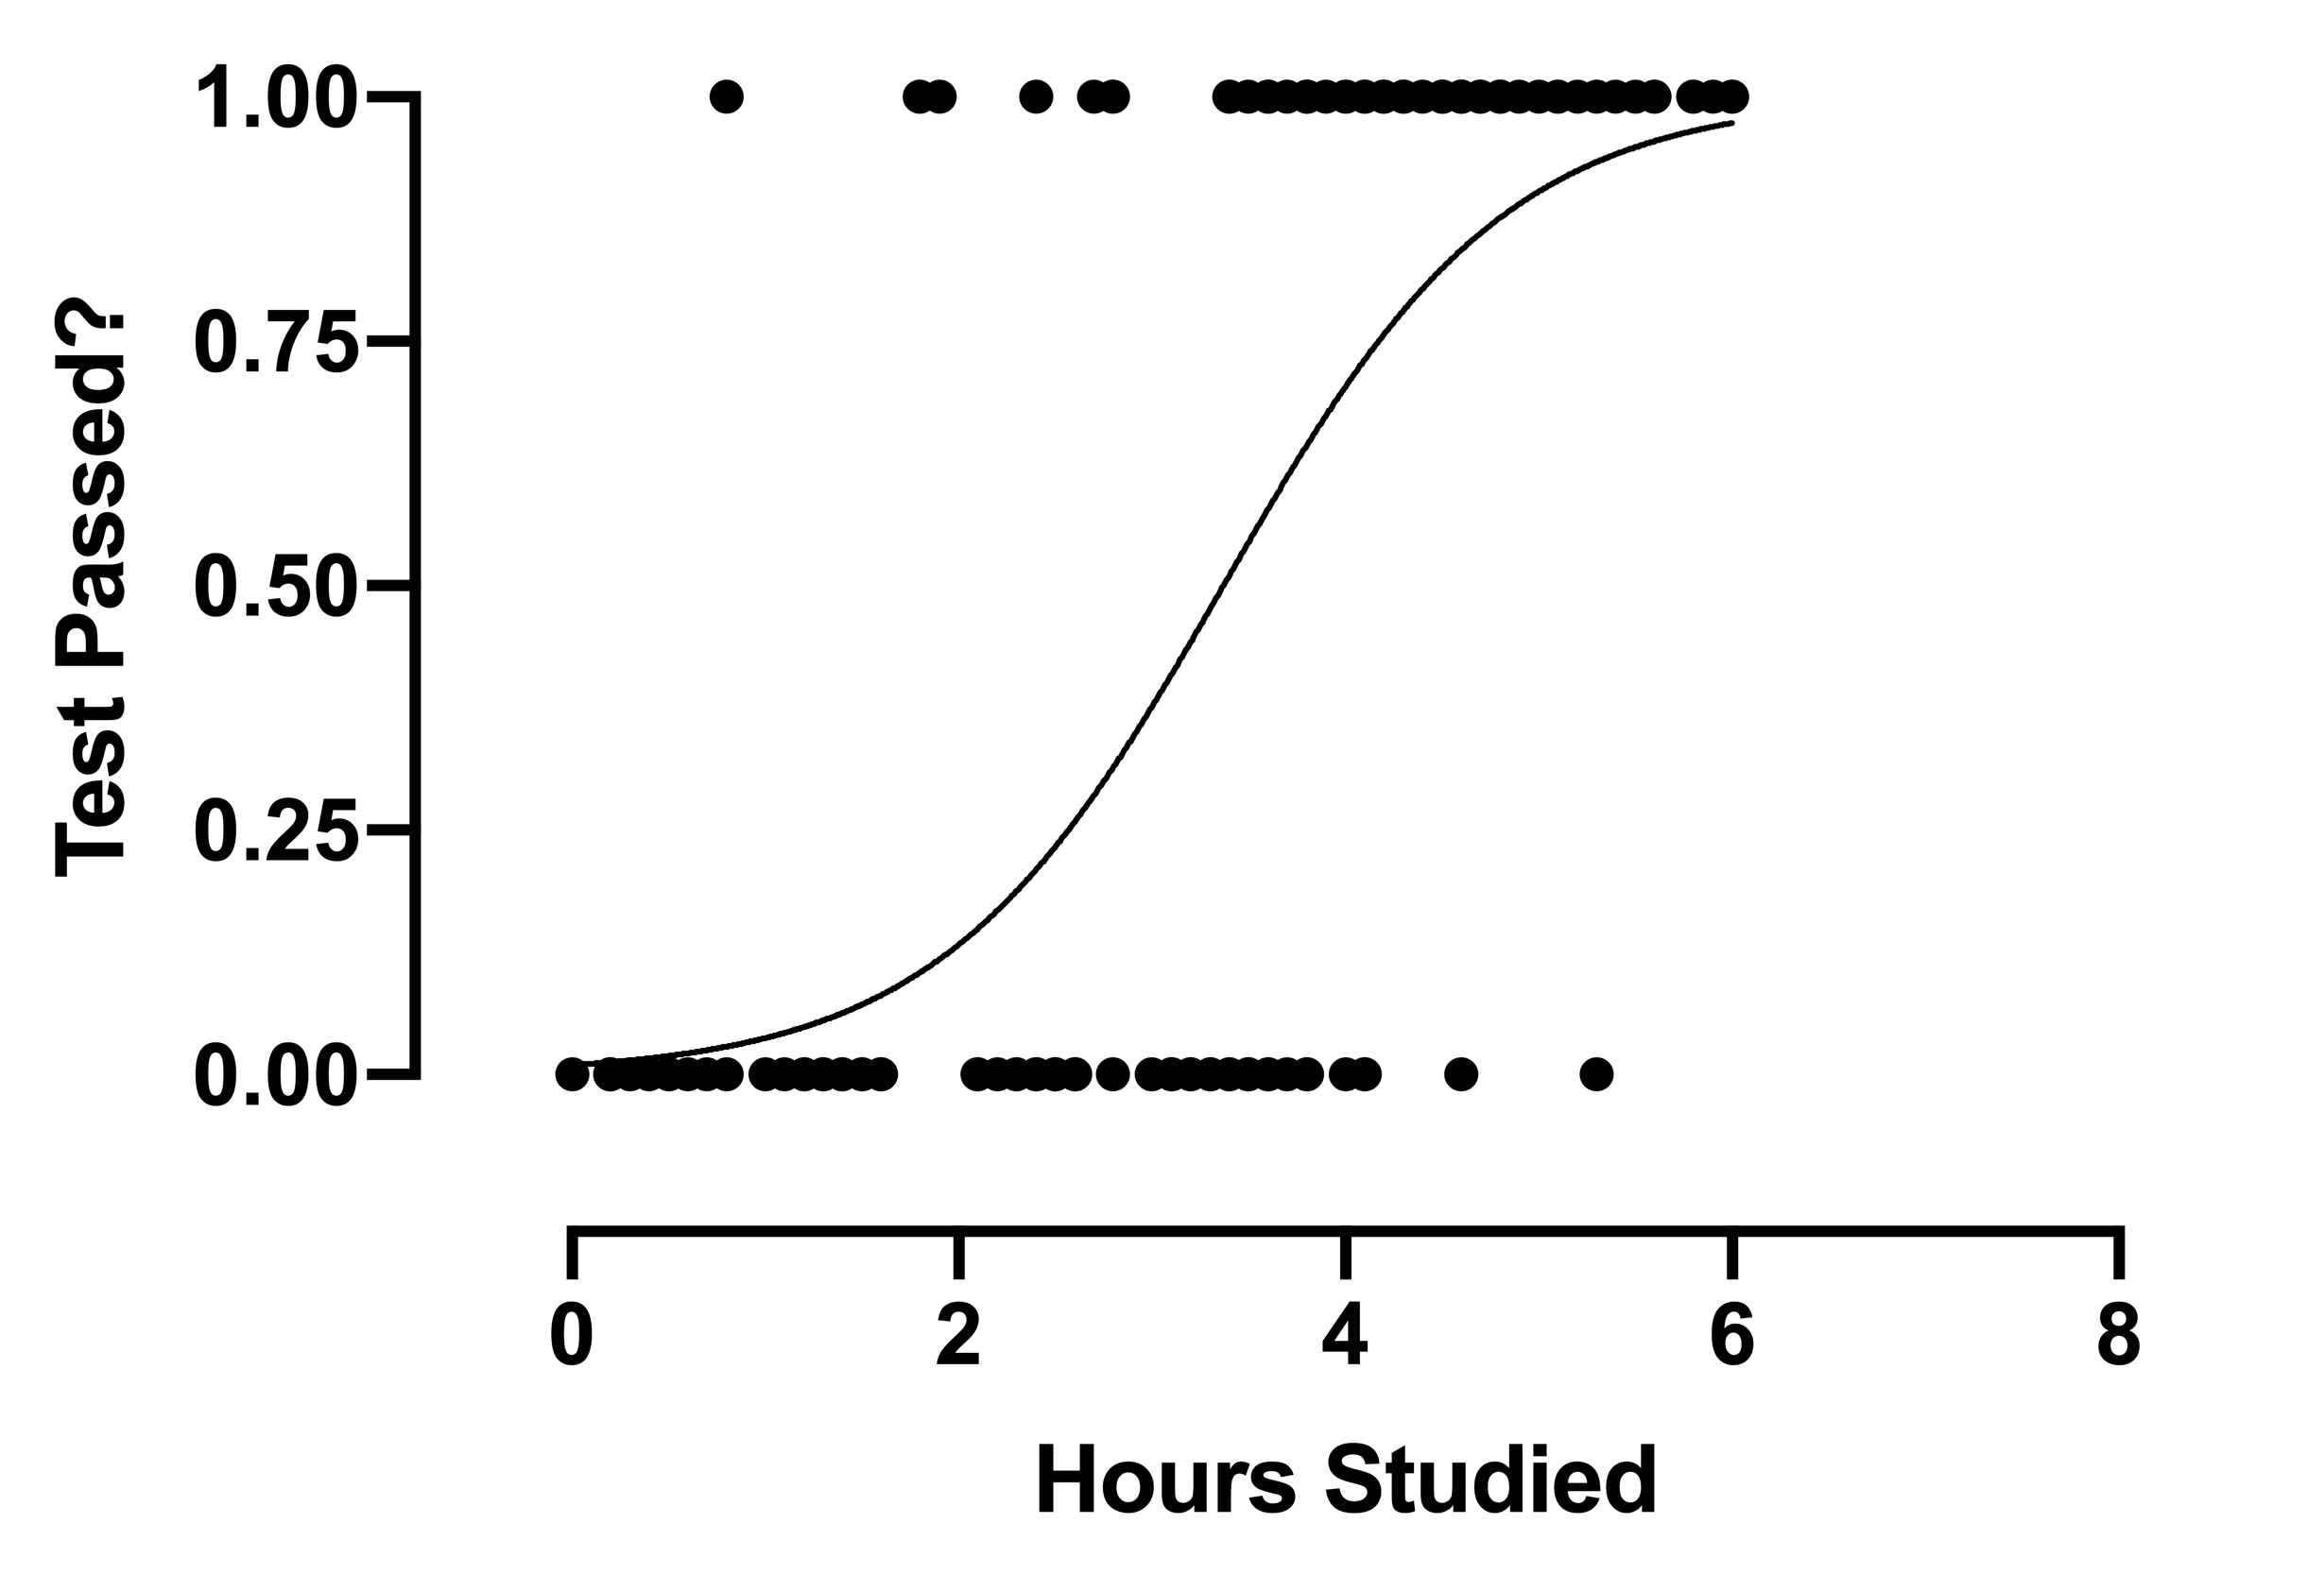
\includegraphics[width=\linewidth]{images/3.fejezet/LogisticRegression.png}
    \caption{Logisztikus regresszió \cite{logisztikusregresszio_abra}}
    \label{fig:logisztikusregresszio}
\end{figure}

\subsection{K-nearest Neighbour Classifier (K-legközelebbi szomszédon alapuló osztályozás)}
Ez az algoritmus azt feltételezi, hogy az azonos kimeneteknek a bemenetei adatai egy koordináta rendszerben ábrázolva közel helyezkednek el egymáshoz képest hiszen hasonlóak \cite{k_legkozelebbi_2}. Ez nem egy modellt épít, hanem eltárolja a tanulásra létrehozott adathalmazt. A kimeneti osztályt az alapján határozza meg, hogy az elmentett adathalmazon belül a szomszédságában milyen osztállyal rendelkező adatok vannak. A K azt határozza meg az algoritmusban, hogy az első hány legközelebbi szomszédját nézze az algoritmus ami alapján dönt \cite{k_legkozelebbi_1}. Példával szemléltetve látható a K-legközelebbi szomszédon alapuló algoritmus a \ref{fig:klegkozelebb} ábrán.

\subsubsection{K-legközelebbi szomszédon alapuló osztályozás előnyei}
\begin{itemize}
    \item Egyszerű algoritmus, amit könnyű implementálni.
    \item Nincs szükség modellt tanítani.
    \item Lehet osztályozásra és regresszióra is használni.
\end{itemize}

\subsubsection{K-legközelebbi szomszédon alapuló osztályozás hátrányai}
\begin{itemize}
    \item Ahogy nő az adat mennyisége úgy egyre-egyre jobban lassul az algoritmus. Nagy adathalmazoknál a lassab algoritmusok közé tartozik.
    \item Nem egyensúlyban lévő kimeneti osztályokkal rendelkező adathalmazokkal problémába ütközik.
    \item A hiányzó adatokkal nem tud mit kezdeni \cite{k_legkozelebbi_1}.
\end{itemize}


\begin{figure}[h]
    \centering
    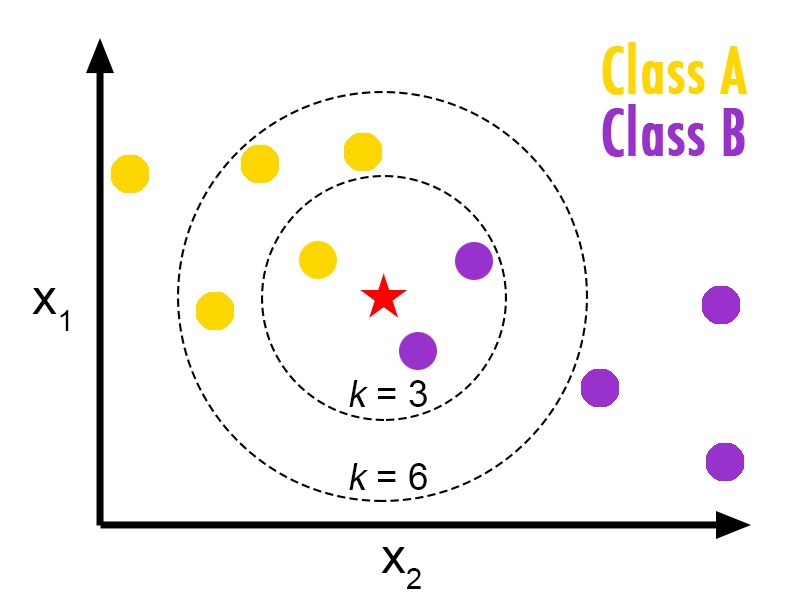
\includegraphics[scale=0.4]{images/3.fejezet/KNearestNeighbours.png}
    \caption{K-legközelebbi szomszédon alapuló osztályozási algoritmus K=3 és K=6 paraméterekkel szemléltetve \cite{klegkozelebbi_abra}}
    \label{fig:klegkozelebbi}
\end{figure}

\subsection{Gradient Boosting Classifier}
Hasonlít a véletlen erdő algoritmushoz, hiszen általában itt is döntési fák sokasága adja a kimeneti osztályt \cite{gradient_boosting_1}. A különbség a kettő között az, hogy míg a véletlen erdő az összes döntési fát egyszerre külön-külön tanítja az adathalmaz egy véletlenszerű mintájából, addig a Gradient Boosting egyszerre csak egy fát épít ami az előző hibáit próbálja orvosolni. Sok lefutás után lesz egyre több döntési fánk egy Gradient Boosting algoritmusban. A legtöbb esetben nem olyan mélyek a döntési fák, mint a véletlen erdő esetében \cite{gradient_boosting_2}. A \ref{fig:gradientboosting} ábrán a Gradient Boosting Classifier egy példája látható.

\subsubsection{Gradient boosting előnyei}
\begin{itemize}
    \item Nem egyensúlyban lévő kimeneti osztályokkal rendelkező adathalmazon is jól működik.
    \item Jobb "tanuló" mint a véletlen erdő.
    \item Tudja kezelni a hiányzó adatokat.
\end{itemize}


\subsubsection{Gradient boosting hátrányai}
\begin{itemize}
    \item Lassab "tanuló", mint a véletlen erdő.
    \item Mivel az egyes döntési fák nem mélyek, így sokra van belőlük szükség, emiatt memória- és időigényes az algoritmus.
    \item Mivel minden hozzáadott döntési fával a saját hibáit akarja javítani, ezért a kiugró értékekre nagy hangsúlyt fektett, emiatt túltanulásra hajlamos \cite{gradient_boosting_2}.
\end{itemize}

\begin{figure}[h]
    \centering
    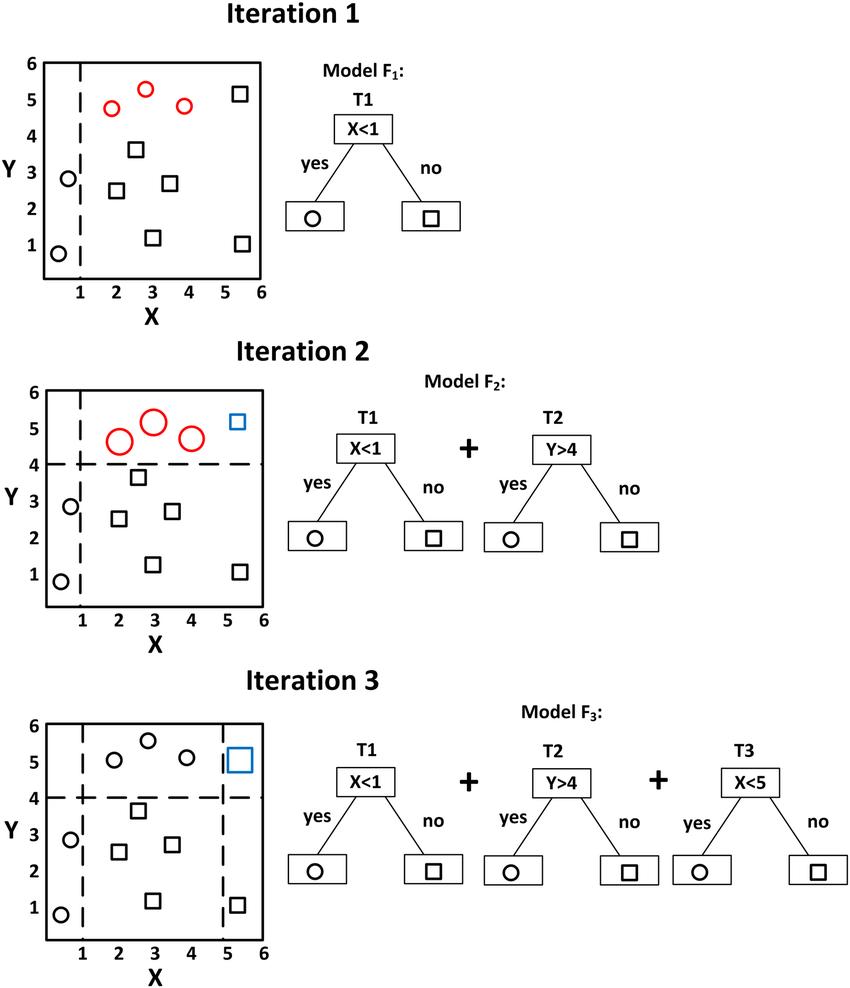
\includegraphics[scale=0.22]{images/3.fejezet/GradientBoosting.png}
    \caption{Gradient boosting tanulása szemléltetve \cite{gradient_abra}}
    \label{fig:gradientboosting}
\end{figure}